%\chapter{Architektur}
\chapter{\colorbox{yellow}{Architektur}}

\section{Konzept}
In diesem Kapitel wird ein Konzept sowie seine Umsetzung für gut skalierbare Webanwendungen ausgearbeitet.

\subsection{Einführung}

\begin{wrapfigure}{r}{0.37\textwidth}
\begin{center}
\vspace{-35pt}%
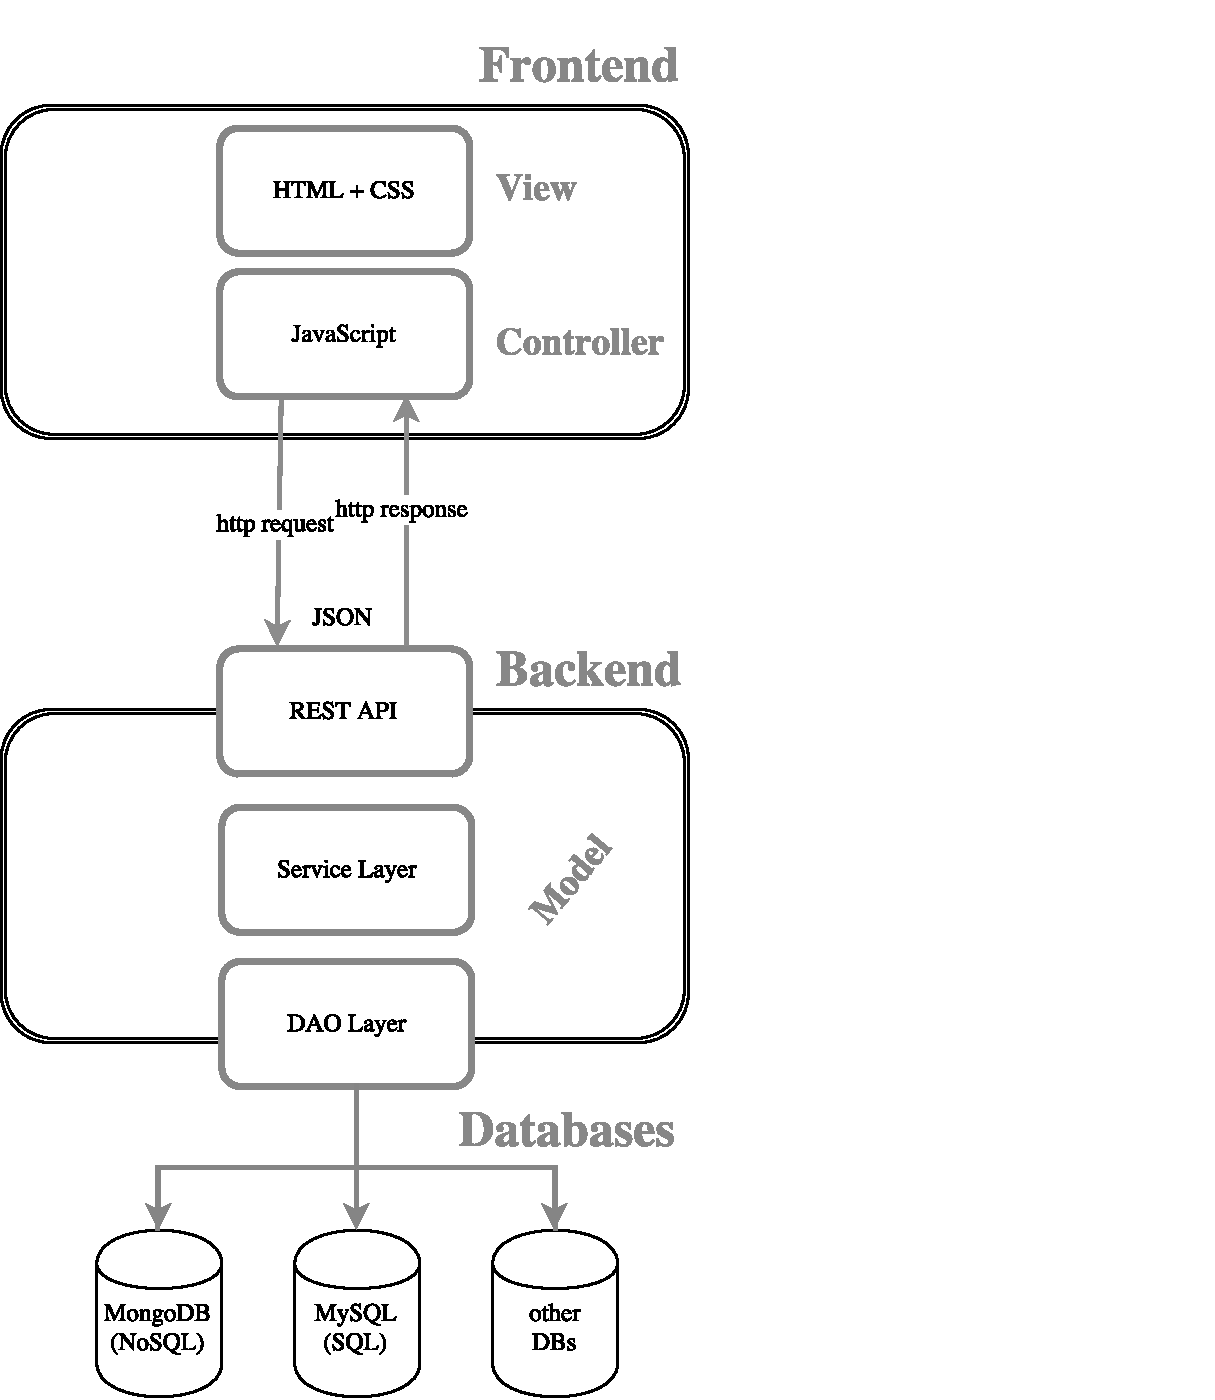
\includegraphics[trim = 0mm 0mm 0mm 0mm, clip, width=0.3\textwidth]{resources/architectureMyAppWithoutFrameworks}
\caption[Architektur-Prototyp]{Architektur-Prototyp}
\label{img:architectureMyApp}
\vspace{-35pt}%
\end{center}
\end{wrapfigure}
Die typische \textbf{MVC}-basierte Architektur einer Webanwendung ist in der Abbildung \ref{img:architectureMyApp} abgebildet.

Der Web-Client, bestehend aus View und Controller wird auf dem Rechner des Anwenders ausgeführt, z. B. in der Browser-Anwendung. Es gibt einen Server (Backend) mit dem der Web-Client kommuniziert, um die Daten abzufragen oder zu ändern. Der Backend-Teil nutzt eine Datenbank, um die Daten persistent zu speichern. Es wird angenommen, dass die Webapplikation für eine große Anzahl von Internetnutzern ausgelegt ist. Das Ziel ist, dass unabhängig von der Anzahl der Nutzer, die die Webanwendung gleichzeitig nutzen wollen, die Webanwendung die konstante Antwortzeiten hat. In dieser Architektur gibt es zwei Komponenten, die bei der steigenden Anzahl von Usern die Antwort verlangsamen können:

\begin{itemize}

\item der Backend-Server, der eine begrenzte Anzahl von \textbf{HTTP}\footnote{\textbf{HTTP} ist ein zustandloses Protokoll zur Übertragung der Daten zwischen Web-Client (=Browser Anwendung) und Web-Server. Jede neue Anfrage, die vom Web-Client erfolgt, erfordert einen neuen Verbindungsaufbau und erneute Datenbeschaffung.}-Anfragen bearbeiten kann. Es ist auch denkbar, dass der Backend-Server auch Geschäftslogik implementiert und auch dafür die  Ressourcen zusätzlich aufwenden muss und

\item die Datenbank. Die Datenbank kann nur eine bestimmte Anzahl der Abfragen gleichzeitig beantworten.

\end{itemize}

Demzufolge, um die konstante Antwortzeiten der Webanwendung bei der steigenden Anzahl von Usern beizubehalten, ist eine Skalierungsstrategie für diese beide Komponente notwendig. Es reicht nicht nur eine zu skalieren, weil dann letztendlich die andere Komponente zum Flaschenhals wird.

Es wird für eine horizontale Skalierung für beide Komponenten entschieden, weil die vertikale Skalierung ihre Grenzen hat.

\subsection{Überblick}

\begin{wrapfigure}{l}{0.42\textwidth}
\begin{center}
\vspace{-20pt}%
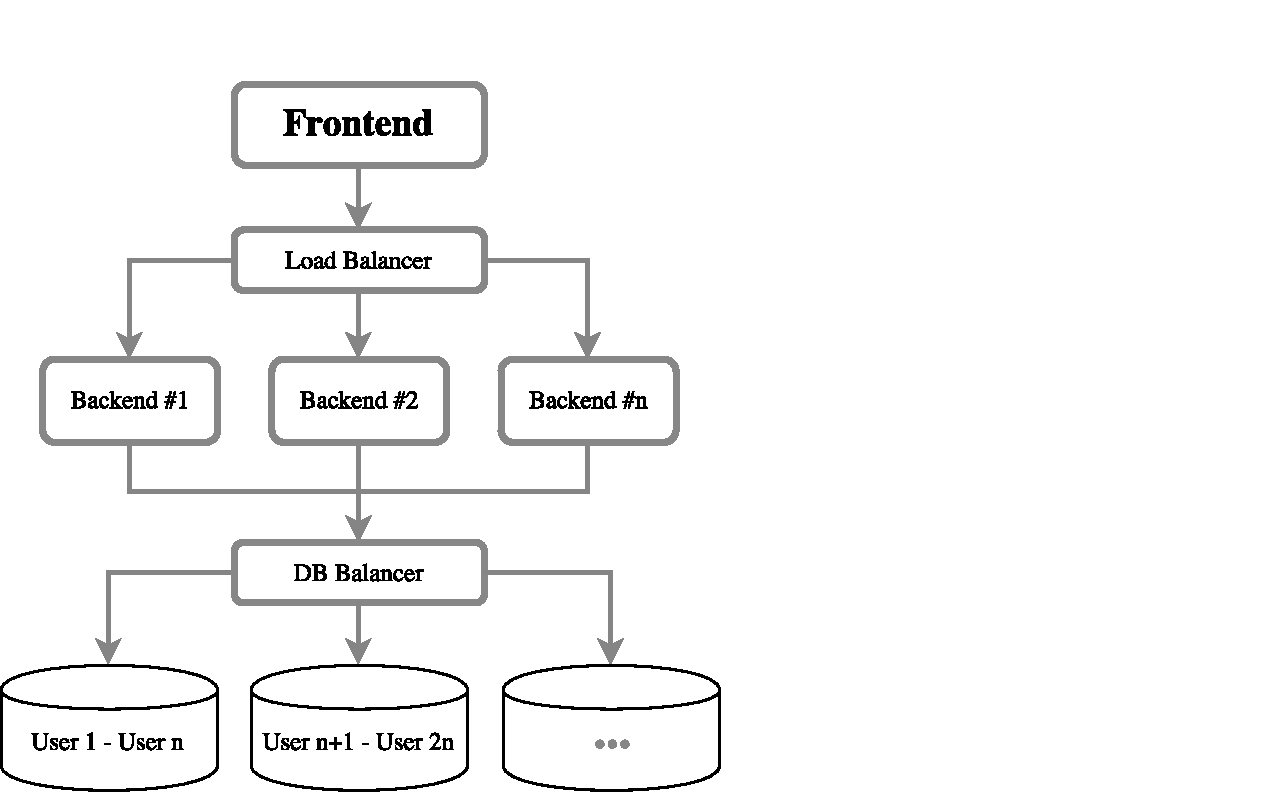
\includegraphics[trim = 0mm 0mm 0mm 0mm, clip, width=0.4\textwidth]{resources/ueberblickArchitektur}
\caption[Überblick zur vorgeschlagenen Architektur]{Überblick zur vorgeschlagenen Architektur}
\label{img:ueberblickArchitektur}
\vspace{-30pt}%
\end{center}
\end{wrapfigure}

%\begin{figure}[H]
%\centering
%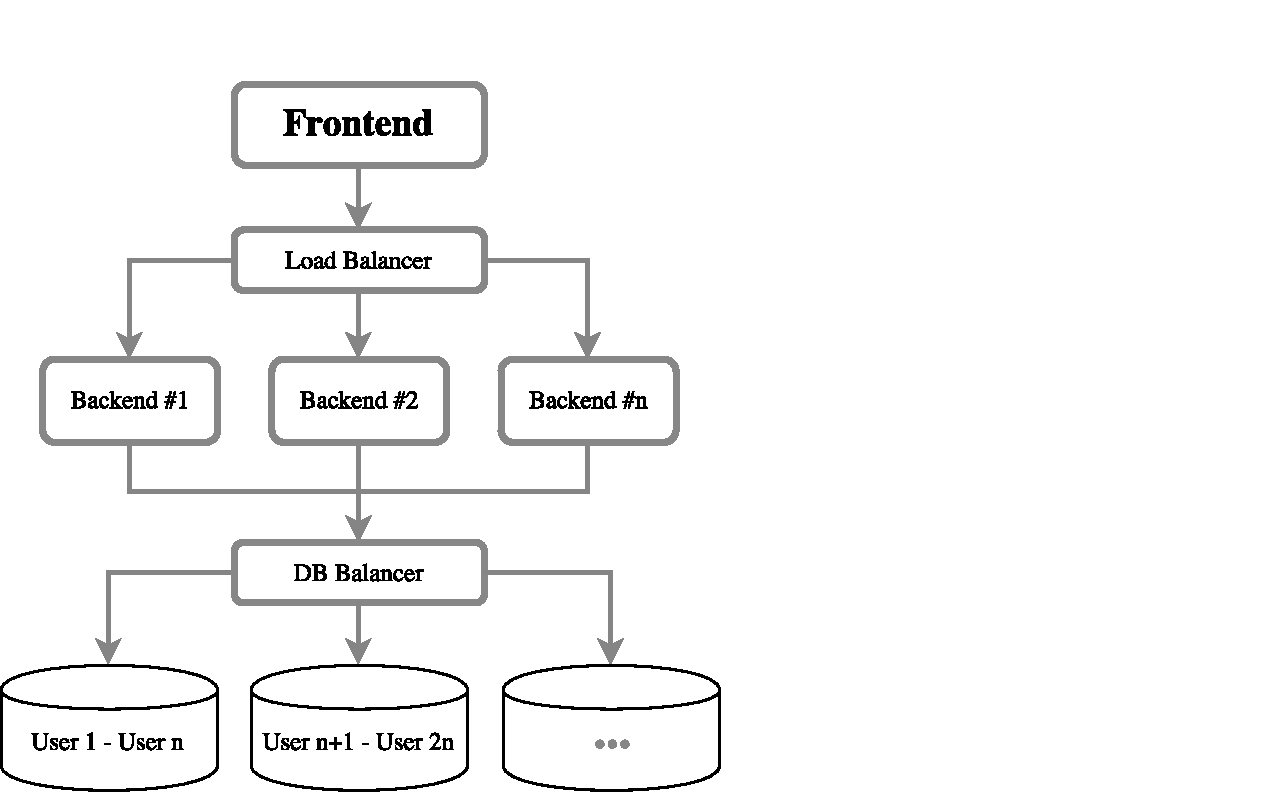
\includegraphics[trim = 0mm 0mm 0mm 0mm, clip, width=0.4\textwidth]{resources/ueberblickArchitektur}
%\caption[Überblick zur vorgeschlagenen Architektur]{Überblick zur vorgeschlagenen Architektur}
%\label{img:ueberblickArchitektur}
%\end{figure}

\textit{Load Balancer}\footnote{Load Balancer, \url{https://f5.com/glossary/load-balancer}, zugegriffen am 21.02.2017} gilt als ein Verteiler, der die Web-Client Anfragen entgegennimmt und sie an mehrere parallel laufende Server verteilt, je nach Maschinenüberlastung. Dabei berücksichtigt \textit{Load Balancer}, dass die Last an Servern gleichmäßig verteilt wird, um die Anwendungs-Performance zu verbessern.

Der Zugriff auf Funktionen in Backend-Teilen erfolgt über \textit{REpresentational State Transfer} oder kurz \textbf{REST}. Durch die Verwendung von REST erfolgen die Web-Client-Anfragen auf Basis des \textbf{HTTP}-Protokolls. Der Web-Client sendet HTTP-Request und erwartet HTTP-Response, in dem Fall des implementierten Prototyps im \textit{JSON}\footnote{JSON (JavaScript Object Notation), \url{http://www.json.org}}-Format.

Der Zustand \textit{(=Session)} der Web-Client-Anfragen wird im Frontend-Teil implementiert und der Web-Server enthält keine Information über Session, da dieser \textit{stateless} arbeitet. \textit{Stateless} bedeutet, dass die Web-Clients mit jeder Anfrage einen neuen Verbindungsaufbau und erneute Datenbeschaffung erfordern und diese voneinander unabhängig sind. Gleich nach einer Web-Server Response wird die Verbindung geschlossen und der Zustand bleibt nicht gespeichert. Somit ist bei einer \textit{stateless-}Webanwendung Sessions nicht möglich.

Falls nach dem Anwendungskontext eine Zustandsspeicherung gefordert wird, wäre die Umsetzung in einer \textit{stateful}-Webanwendung möglich. Bei einer \textit{stateful}-Webanwendung werden Web-Client Anfragen zu einer gemeinsamen logischen Sitzung zusammengefasst, um alle Nutzerinteraktionen hinweg in einem einzigen Kontext auszuführen. Dies wird mithilfe von \textit{Session-Cookies}\footnote{Session-Cookie, \url{https://help.sap.com/erp2005_ehp_04/helpdata/de/cc/d6eef928f711d5991f00508b6b8b11/content.htm}, zugegriffen am 20.01.2017} realisiert.

Bei \textit{stateful}-Anwendungen muss der \textit{Load Balancer} so konfiguriert sein, dass alle von einem Web-Client kommenden Requests an einen Server weitergeleitet werden können, was komplexer ist, als bei \textit{stateless}-Anwendungen. 

Die eigentliche horizontale Skalierung der Daten findet auf der Datenbankebene statt. Die Daten werden in die Datenbank ständig geschrieben und gelesen. Um bei diesen Prozessen eine gute Performance auch auf Datenbankebene zu erreichen, wird angeboten, die Daten auf Knoten zu verteilen. Für weitere Requests wird eine Komponente geben, die anhand der Informationen in Requests erkennen wird, wo genau die Daten abgelegt sind. 
%- WriteConcern in MongoDB: abhängig vom Anwendungskontext, ob in dieser mehr write oder mehr read-Operationen durchgeführt werden, muss mongoDB so konfigutiert werden, dass die Anfragen gut skalierbar sind. Es ist möglich, die Read-Operationen bei Secondaries zu aktivieren, dabei muss man aber auch den Ablauf der Transaktion so zu konfigurieren, dass die Transaktion erst dann abgeschlossen ist, wenn die Daten auf allen Knoten repliziert sind, danach wird die Transaktion als abgeschlossen gezählt.

%\begin{wrapfigure}{r}{0.4\textwidth}
%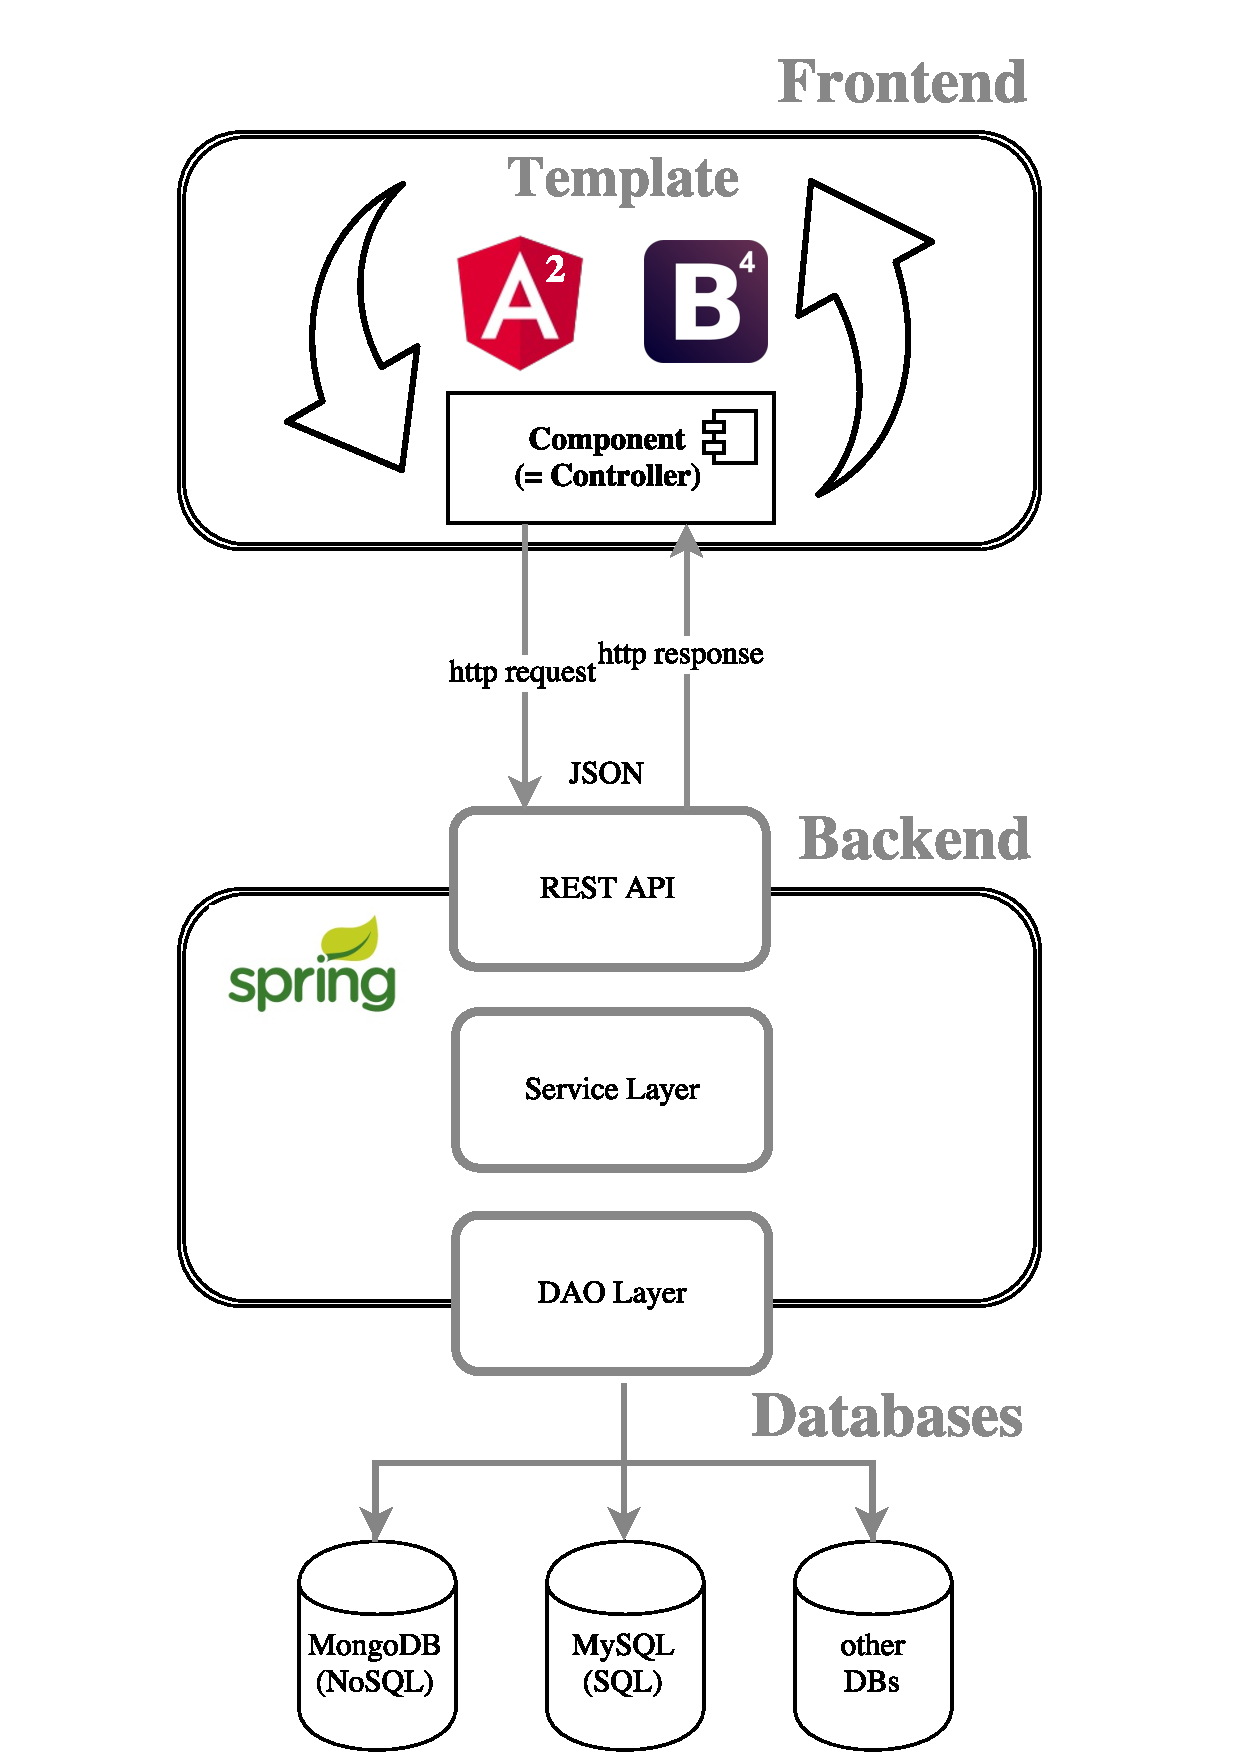
\includegraphics[trim = 20mm 0mm 30mm 9mm, clip, width=0.4\textwidth]{resources/architectureMyApp}
%\caption[Architektur-Prototyp]{\label{img:myArchitecture}Architektur-Prototyp}
%\end{wrapfigure}

%\section{Datenhaltungsschicht (Databases)}
\section{Umsetzung}




